%% LyX 2.3.3 created this file.  For more info, see http://www.lyx.org/.
%% Do not edit unless you really know what you are doing.
\documentclass[12pt,english]{article}
\usepackage{ae,aecompl}
\usepackage[T1]{fontenc}
\usepackage[latin9]{inputenc}
\usepackage{geometry}
\geometry{verbose,tmargin=3cm,bmargin=3cm,lmargin=2.5cm,rmargin=2.5cm}
\usepackage{float}
\usepackage{textcomp}
\usepackage{url}
\usepackage{amstext}
\usepackage{amssymb}
\usepackage{graphicx}
\usepackage{setspace}
\usepackage{esint}
\usepackage[authoryear]{natbib}
\doublespacing

\makeatletter
%%%%%%%%%%%%%%%%%%%%%%%%%%%%%% User specified LaTeX commands.
\usepackage{aecompl}\usepackage{lineno}

\usepackage{babel}

%\linenumbers

\makeatother

\usepackage{babel}
\begin{document}
\title{Looking for compensation at multiple scales in a wetland bird community}
\author{{\Large{}{}Fr�d�ric Barraquand$^{1,2,*}$, Coralie Picoche$^{1}$,
Christelle Aluome$^{1,3}$, }\\
 {\Large{}{}Laure Carassou$^{1,4}$ \& Claude Feign�$^{5}$}}

\maketitle
{\large{}{}\bigskip{}
}{\large\par}

{\large{}{}}\textsuperscript{{\large{}{}1}}{\large{}{}~University
of Bordeaux, Integrative and Theoretical Ecology, LabEx COTE, B�t.
B2 - All�e Geoffroy St-Hilaire, 33615 Pessac, France \bigskip{}
}{\large\par}

{\large{}{}}\textsuperscript{{\large{}{}2}}{\large{}{}~CNRS, Institute
of Mathematics of Bordeaux, 351 Cours de la Lib�ration, 33405 Talence,
France}{\large\par}

{\large{}{}\bigskip{}
}{\large\par}

{\large{}{}}\textsuperscript{{\large{}{}3}}{\large{}{}~ISPA, Bordeaux
Sciences Agro, INRA, 33140 Villenave d'Ornon, France}{\large\par}

{\large{}{}\bigskip{}
}{\large\par}

{\large{}{}}\textsuperscript{{\large{}{}4}}{\large{}{}~Irstea,
UR EABX, 50 Avenue de Verdun, 33612 Cestas, France}{\large\par}

{\large{}{}\bigskip{}
}{\large\par}

{\large{}{}}\textsuperscript{{\large{}{}5}}{\large{}{}~PNR Landes
Gascognes, Teich Ornithological Reserve, Rue du Port BP 11 33470 Le
Teich, France}{\large\par}

{\large{}{}\bigskip{}
}{\large\par}

{*} Corresponding author. Email: frederic.barraquand@u-bordeaux.fr

\thispagestyle{empty}

\pagebreak{}

%\linenumbers

\begin{linenumbers}{
\begin{abstract}
1. Compensatory dynamics, during which community composition shifts
despite a near-constant total community size, are usually rare: synchronous
dynamics prevail in natural communities. This is a puzzle for ecologists,
because of the key role of compensation in explaining the relation
between biodiversity and ecosystem functioning.

2. However, most studies so far have considered compensation in either
plants or planktonic organisms, so that evidence for the generality
of such synchrony is limited. Here, we extend analyses of community-level
synchrony to wetland birds.

3. We analyse a 35-year monthly survey of a community where we suspected
that compensation might occur due to changes in water levels, favouring
birds with different habitat preferences, and potential competition.
We perform both yearly analyses by season, using a synchrony index,
and monthly analyses using wavelet-based measures allowing for scale-dependence.
We analyse synchrony both within and between guilds, with guilds defined
either as tightknit phylogenetic groups or larger functional groups.

4. We find that abundance compensation is rare, likely due to the
synchronizing influence of climate on birds, even after considering
several temporal scales of covariation (during either cold or warm
seasons, above or below the seasonal scale). Negative covariation
in abundance at the whole community level did only appear after a
management change in the reserve, and at the scale of a few months
or several years. We also found that synchrony varies with taxonomic
and functional scale: the rare cases where compensation appeared consistently
at the annual scale were \emph{between} rather than \emph{within}
guilds, using functional groups.

5. Although most research has focused on viewing compensation vs synchrony
across temporal scales, because synchrony is guaranteed at the temporal
scale of the dominant environmental forcing, our results suggest that
compensation can be masked as well at some taxonomic or functional
scales. We suggest that abundance compensation may have more potential
to emerge between broad functional groups, rather between species.
\end{abstract}
\textbf{Keywords: }compensation; synchrony; biodiversity; birds; time
series; wavelets

\newpage{}

\section*{Introduction}

Density compensation occurs when individuals of a given species replace
individuals of other species within a community, either because of
explicit competitive processes or shifts in environmental drivers
that change selection pressures \citep{gonzalez2009causes}. The community
as a whole then exhibits lower biomass variation than its constituent
species \citep{gross2013species}: some degree of compensation or
asynchrony is therefore a prerequisite to stabilization at the community
level \citep{loreau2013biodiversity}.

Understanding why environmental variation may lead to compensation
is relatively easy: if species have different environmental preferences
(e.g., thermal optima), and the environment changes over time, different
species will be fittest at different points in time. As a consequence,
relative abundances will shift over time even though the community
biomass as a whole may remain relatively stable \citep{gonzalez2009causes}.
However, the conditions for compensation to happen also depend on
the particulars of the interactions between and within species in
the community.

Compensation is particularly likely to occur when such temporal environmental
variation combines with a space or strongly limiting resource constraint,
so that individuals are close to competing in a zero-sum game (sensu
\citealp{hubbell2001unified} or lottery-style models, \citealp{chesson_multispecies_1994}).
When the total community size is constant over time, and the composition
fluctuates, negative covariation between abundances then emerges by
design \citep{loreau_species_2008} since no species can increase
without another species decreasing in abundance. Outside of this zero-sum
scenario, in models where Lotka-Volterra competition is combined with
temporal environmental variability, theoretical research has revealed
that increased interspecific competition might not increase species
compensation \citep{ives_stability_1999} and might even decrease
it \citep[i.e., increase species synchrony instead,][]{loreau_species_2008,loreau2013biodiversity},
though this depends on the fluctuation regime. Thus, in a world where
total community size varies, predicting whether compensatory (or asynchronous)
 dynamics can occur is intrinsically difficult \citep{klink_functional_2019}.

Early investigations of the frequency of synchronous vs compensatory
dynamics focused on the variance ratio, that is, the variance of the
sum of the community biomass divided by the sum of the variance of
the component species biomasses \citep{houlahan_compensatory_2007,gonzalez2009causes}.
Unfortunately, this metric is not appropriate for communities subjected
to community-wide environmental forcing \citep{ranta_detecting_2008},
because a main environmental driver (e.g., temperature or light) may
synchronize species abundances or growth rates at some scale, creating
large variance in community-wide biomass, in spite of strongly competitive
dynamics. Further research has therefore focused on specific timeframes
during which compensatory dynamics may be found (e.g., below the seasonal
scale at which temperature fluctuations tend to synchronize species
dynamics, \citealp{vasseur_synchronous_2014}).

Despite efforts to look for more meaningful temporal scales in community-level
time series, temporal compensation has remained surprinsingly elusive
in the field \citep{houlahan_compensatory_2007,vasseur_synchronous_2014};
but see \citet{ernest2008zero,christensen2018long}. Most datasets
used so far to evaluate temporal compensation vs synchrony involve
planktonic organisms \citep{vasseur2007spectral,vasseur_synchronous_2014}
or terrestrial plants (\citealp{houlahan_compensatory_2007,gross2013species};
though see \citealp{bell_stability_2014} in fishes and \citealp{klink_functional_2019}
in beetles). Here, we take advantage of a long-term bird abundance
time series record at the monthly scale (over 35 years), in a natural
reserve, allowing us to dig deeper into patterns of synchrony, at
several temporal and taxonomic or functional scales.

Indeed, taxonomic and functional scales should be main modulators
of synchrony/compensation. On the one hand, compensation can be high
between similar and closely related species. If two species of ducks
A and B share almost the same niche, individuals from either species
experience similar competition from species A or B, and should feel
the effects of other species in the community identically. This favours
priority effects \citep{fukami_historical_2015}, with chance due
to movement events determining whether species A or B locally dominates,
which can then provide compensation at the landscape level \citep{loreau2003biodiversity}.
On the other hand, it could be argued that these two similar duck
species will precisely respond in similar ways to environmental variables,
which tends to obfuscate compensation. Hence, more dissimilar species
or groups (within the same trophic level nonetheless) could exhibit
more compensation \citep{morin2014temporal,klink_functional_2019}
because they are more likely to respond to the environment in an asynchronous
manner (\emph{sensu} \citealp{loreau2013biodiversity}). Surprisingly,
such compensation \textit{between} guilds has been less well explored
empirically than \emph{within} guilds, even though there is actually
some empirical evidence for compensation between dissimilar guilds
\citep[e.g.,][]{roscher_identifying_2011,sinclair2013asynchronous,klink_functional_2019}.
In this paper, we explore the level of compensation/synchrony within
or between guilds of a wetland bird community, along either taxonomic
or functional classifications. Although a functional classification
might appear intuitively more appealing, our knowledge of functional
traits is necessarily partial and imperfect, so that a taxonomic description
can sometimes be preferable \citep{clark_why_2016}.

Our objective is therefore to examine how synchronous or compensatory
bird communities are at different temporal and taxonomic (or functional)
scales. Our dataset is ideally suited to the task given that (i) it
is a highly temporally resolved time series with respect to the species
typical generation times, but it also extends well beyond generation
time (35 years) and (ii) the reserve where the data has been collected
was subjected to a major management change c. 2006 (change in water
levels), favouring different types of wetland birds (so that over
long timescales, there is a real potential for changes in community
composition).

\section*{Material and Methods}

\subsection*{Data}

The monthly time series used for the statistical analyses have been
collected at the Teich Ornithological Reserve, Arcachon Bay, France
(44.64�N / -1.02�E), by the staff of the Teich reserve, over the whole
study period. A species list of the frequent birds is provided in
SI Appendix S1. The reserve comprises 120 ha of wetlands, and the
counts have been aggregated at the reserve scale (summed over 18
sectors where the counts are actually performed, using binoculars).
We use for each species the maximum observed abundance over a month,
which provides a ``monthly snapshot'' of the bird abundance, that
has been used to monitor the reserve since its inception. When abundance
values are missing for certain species and months, we replace them
by 0s. Given the sustained observation effort (all sectors are patrolled
multiple times throughout the month by the staff, amateur ornithologists
visiting the reserve daily and communicating their findings to the
reserve staff), we consider that the absence of counts for a given
species signals its true absence from the reserve. This creates some
zero abundances for rare species at the monthly scale. We have not
attempted to ``correct'' those zeroes (e.g., inferring the ``missing''
data with a model assuming that our reserve is a subsample of a regional
population) because doing so would have compromised the patterns of
local synchrony/compensation. However, we did check below that having
such zeroes in the monthly time series cannot affect our conclusions.
In the statistical analyses, we use seasonally averaged abundances
(plotted in Fig. \ref{fig:Temporal-trends}), as well as the original
monthly data (presented in Appendix S2). We defined two seasons based
on observations of bird presence. We defined a `warm season', from
May to August, and a `cold season' as the months between November
and February of the following year. From an ecological viewpoint,
this seasonal classification separates wintering birds from summer
residents (some of whom are breeding). This makes sense biologically
because the two communities have different requirements and respond
differentially to abiotic drivers. It is also useful from a more statistical
perspective, as there is a shift in composition between the seasons,
though winter and summer communities partially overlap due to a number
of shared species.

Fig. \ref{fig:Temporal-trends} shows the patterns in abundance for
key groups in the Teich reserve bird community, showing the marked
signature of seasonality.

\begin{figure}[H]
\begin{centering}
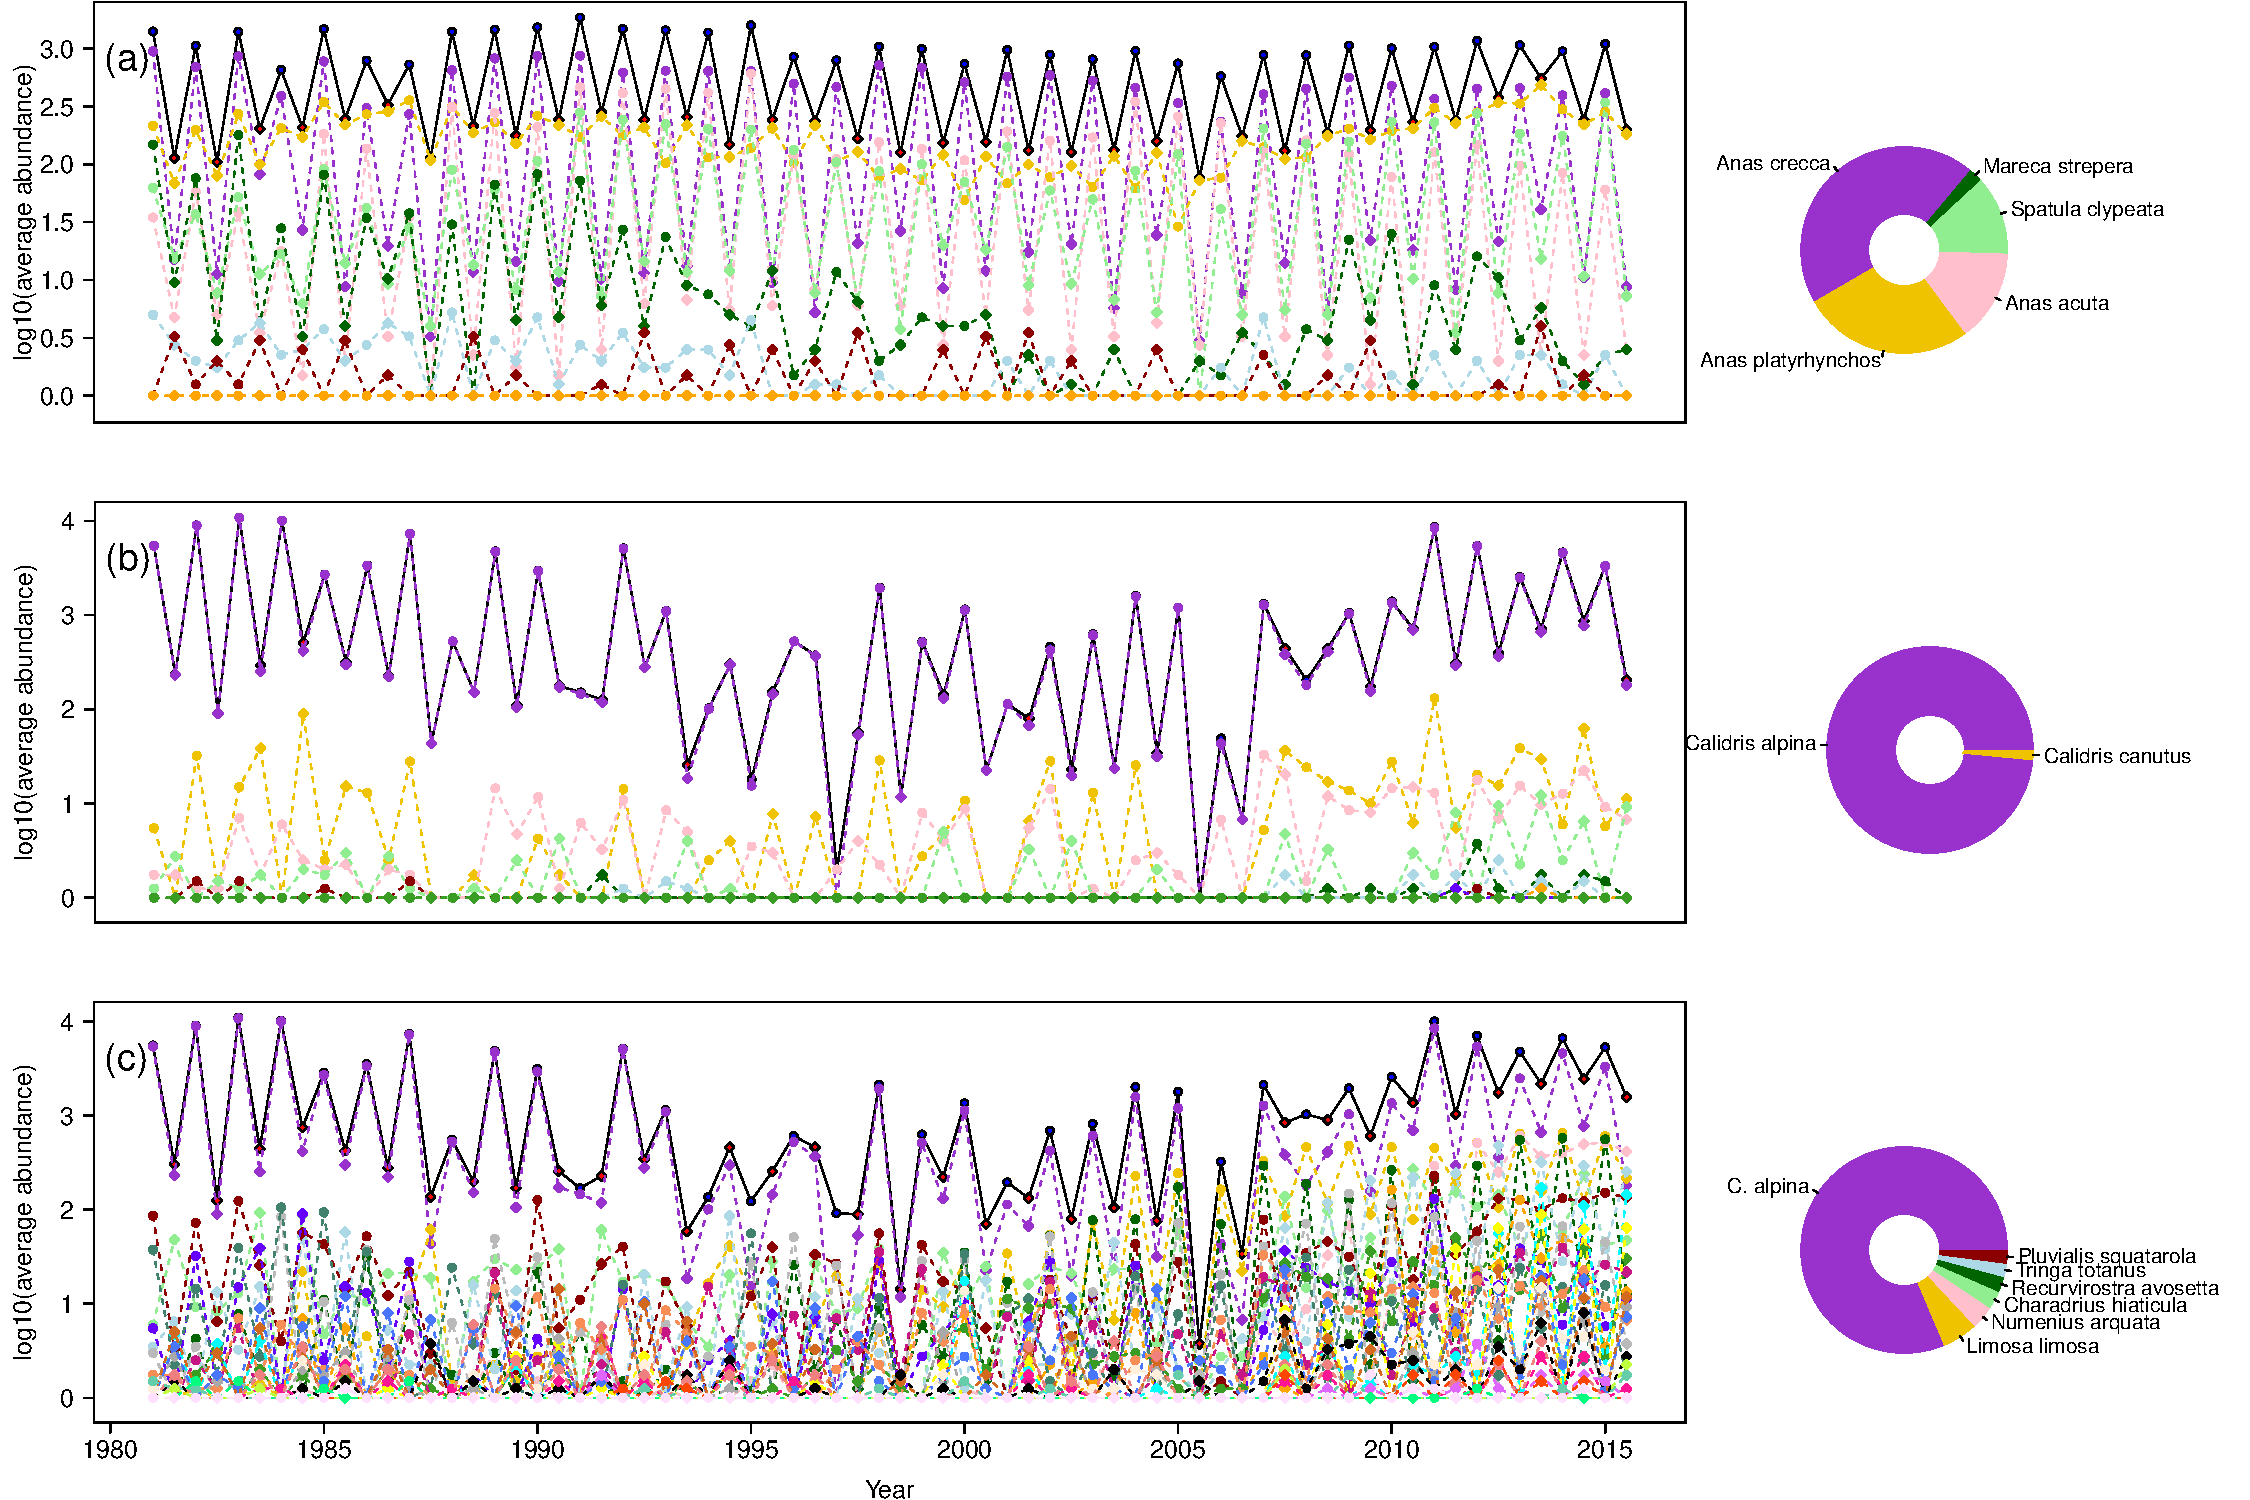
\includegraphics[width=18cm]{average_abundance_timeseries_v2}
\par\end{centering}
\caption{Time series of seasonally averaged abundance for\emph{ }ducks of the
tribe\emph{ Anatini} (a), calidrids (b, \emph{Calidris} genus), and
all waders (c, including calidrids). The solid black lines represent
the summed average abundances for each guild, dotted lines represent
average abundance for each species. Circles represent the cold season
and diamonds, the warm season. The coloured symbols below the curves
represent each species abundances, with species composition on the
right side on the donut plots for the most abundant species (over
1\% of relative abundance in the group considered). \label{fig:Temporal-trends}}
\end{figure}


\subsection*{Bird taxonomic and functional groups}

The reserve is dominated by waders and waterfowl (ducks, geese and
swans). These two functional groups collectively represent 68\% of
the total number of observed birds over the years and are always present
on site. Two fairly common phylogenetic groups, both in abundance
and occurrence, are members of the \emph{Anatini }tribe \citep[corresponding previously to the Anas genus,][]{gonzalez_phylogenetic_2009}
in ducks and members of the \emph{Calidris} genus in waders. Waders
and ducks have different environmental preferences, with ducks (and
waterfowl more generally) preferring water levels allowing them to
dive, while waders usually forage on mudflats. A list of all birds
found frequently in the reserve is presented in Appendix S1; aside
from waders and waterfowl, other common species include herons, egrets
and cormorants (see below). Among the fish eaters, grebes and gulls
were also present; a few raptors as well.

To examine compensation \emph{between} and \emph{within} the waders
and waterfowl categories, we contrasted analyses using a taxonomic
classification of the species (i.e., between and within phylogenetic
groups such as genera) and a functional classification of the species
(26 species of waders vs 17 species of waterfowl). The waterfowl group
includes all anatids (ducks, geese and swans in particular) as well
as the common coot \emph{(Fulica atra}, an abundant species here,
which is a Rallidae but resembles a duck in morphology and foraging
habits; hence its inclusion).

In addition to our main analyses on waders and waterfowl, we also
``zoomed in'' on a set of species that were known to exhibit potentially
compensatory dynamics through competition for roosting sites: the
great cormorant \textit{(Phalacrocorax carbo)}, the little egret (\textit{Egretta
garzetta}) and the grey heron (\textit{Ardea cinerea}). The little
egret and the grey heron abundances were summed because of their similar
requirements (i.e., they form a small functional group).

\subsection*{Statistical Analyses}

\subsubsection*{Yearly analyses}

We used for yearly analyses the synchrony index $\eta$ defined by
\citet{gross2013species}, which is constructed as the mean cross-correlation
between each species biomass and the summed biomasses of the rest
of the community (eq. \ref{eq:Gross}).

\begin{equation}
\text{\ensuremath{\eta}}=\frac{1}{n}\sum_{i}\text{Corr}(X_{i},\sum_{j\neq i}X_{j})\label{eq:Gross}
\end{equation}

where $X_{i}$ is the abundance or biomass of species $i$ in a community
of $n$ species. This synchrony index described in eq. \ref{eq:Gross}
varies between -1 (perfect compensation, total biomass is constant)
and 1 (complete synchrony), while 0 represents a case where all populations
fluctuate independently. Contrary to other indices (e.g., \citet{loreau_species_2008}'s
$\phi$), this index is independent from the richness $n$ of the
community (or more generally the number of system components) and
its overall stability \citep{bluthgen_land_2016,hallett_codyn_2016}.
This is particularly important here as we perform analyses at different
taxonomic scales, and therefore with a different $n$ in eq. \ref{eq:Gross}.

We computed synchrony indices at the year $\times$ season scale using
the codyn package in R \citep{hallett_codyn_2016}. That is, we constructed
two community-level time series where each year is associated to a
vector of species abundances, one for the cold season and one for
the warm season. To do so, we averaged monthly bird abundances, for
each species, over the season duration. We then computed the synchrony
index for both cold and warm seasons using the year as our statistical
unit. In follow-up analyses, we also differentiated periods before
and after 2006, given that a management change occurred within the
reserve in 2006. We considered both the synchrony inside a given group
(e.g., among species of the \textit{Calidris} genus) or between groups
(e.g., between the summed abundances of the 7 species of tribe \textit{Anatini}
and\emph{ }\textit{\emph{the sum of the 7 }}\textit{Calidris} species).
In the latter case of between-groups comparisons, we summed species
together before seasonal averaging, to consider seasonal averages
of the monthly group-level abundance.

We computed the statistical significance of the synchrony index by
comparing the observed values to the distribution of $\eta$ under
the null hypothesis \citep{gouhier_synchrony_2014}, which amounts
to zero cross-correlations between species abundances (or guild-level
abundances when considering functional groups). The challenge, in
order to construct such null hypothesis, is to remove all cross-correlations
while keeping the exact same autocorrelation in each individual time
series. Therefore, for each set of time series (each combination year
$\times$ season for a given community), we constructed 100 ``surrogates''
in which we kept auto-correlations but removed cross-correlations
between time series. There are multiple ways to erase cross-correlations
depending on the resolution of the considered community. Within guilds,
we shifted the time-series \citep{purves_fine-scale_2002} while between
guilds (two groups only), we used a frequency-based approach (Iterated
Amplitude-Adjusted Fourier Transform or IAAFT, see \citealp{schreiber_surrogate_2000}).
We first explain the shift-based approach: the suite of abundance
values (after seasonal averaging) is displaced by a random temporal
lag $\tau$, so that a value $y_{t}$ is now found at $y_{t+\tau}$.
At the boundary (the end of the time series), remaining points are
displaced towards the beginning of the time-series, which implements
a toroidal shift. This method works well when comparing many times
series corresponding to the multiple species. However, when computing
synchrony across only two groups (between guilds), spurious cross-correlations
could emerge with a shift-based approach as the number of possible
combinations is more limited. Therefore, to test for synchrony between
the summed abundances of two guilds or taxonomic units, we used the
more sophisticated IAAFT method \citep{schreiber_surrogate_2000},
which retains the frequency spectrum of the time series while randomising
its values. We obtained 100 sets of randomised time series for each
computed synchrony index. We then compared the number of $\eta_{H0}$
values which exceeded or were inferior to the observed value to compute
the p-value \citep{north_note_2002}: we use the ratio $(r+1)/(n+1)$
where $r$ is the number of surrogate values that are $\ge\eta_{obs}$,
respectively $\le\eta_{obs}$, and $n$ is the number of surrogates.
Independence of species was rejected at the 10\% threshold with a
Benjamini-Hochberg correction, as we compare across 2 seasons and
3 periods, with partially overlapping data. This was found satisfactory
based on simulated data, although power is low for detecting compensation
(i.e., the null cannot always be rejected) when only two groups are
compared.

\subsubsection*{Wavelet analyses}

In addition to the time-domain analyses above, we performed frequency-domain
analyses for a range of temporal scales ranging from a few months
to years. This was done in particular for analyzing synchrony within
the rich wader community, as well as the group formed by the great
cormorant, grey heron and little egret. All wavelet analyses take
as input the monthly time series data. Based on the work by \citet{keitt_coherent_2008}
and follow-up by \citet{vasseur_synchronous_2014}, we used the wavelet
transform of the time series to measure the coherency between time
series

\begin{equation}
\rho(t,s)=\frac{\Lambda_{t,s}(|\sum_{k}w_{k}(\tau,s)|)}{\Lambda_{t,s}(\sum_{k}|w_{k}(\tau,s)|)}\label{eq:Keitt}
\end{equation}

where $w_{k}(\tau,s)$ is the continuous Morlet wavelet transform
of species $k$ at time $\tau$ for scale $s$, $\Lambda_{t,s}(\centerdot)=\int_{-\infty}^{+\infty}e^{-\frac{1}{2}(\frac{t-\tau}{s})^{2}}(\centerdot)d\tau$
and $|\centerdot|$ is the modulus of the complex number. The numerator
corresponds to the total abundance variation while the denominator
corresponds to the fluctuations of each species. This index is close
to 0 when species compensate and reaches 1 when they are synchronous.
As before, the significance of each value was tested at the 10\%,
Benjamini-Hochberg corrected, threshold by 100 phase-randomisations
of each species time series, and computation of the corresponding
$\rho$ values. The robustness of the wavelet approach to the presence
of exactly zero values is tested in Appendix S7.

All datasets and statistical analyses are available in a GitHub repository
\url{https://github.com/fbarraquand/BirdTimeSeries_Teich}\footnote{Will be made public upon acceptance}.

\section*{Results}

\subsection*{Synchrony within phylogenetic or functional groups}

Using a taxonomic classification of the community, \textit{\emph{focusing
on the genera}} \textit{Calidris} and tribe \textit{Anatini }\textit{\emph{(formerly
}}\textit{Anas}\textit{\emph{)}} as two key examples of taxonomic
units with contrasted preferences, we can see that within-genus synchrony
dominates at the seasonal scale. Using functional groups (waders and
waterfowl), synchrony within functional groups was also prominent.
The Gross synchrony indices are indeed mostly positive, and always
positive whenever significantly different from the null hypothesis
(no temporal correlation between species). Therefore, there is no
compensation within guilds (Fig. \ref{fig:Gross-synchrony-index}a
and b) at the annual scale. This matches the patterns obtained within
the entire wetland bird community (Appendix S3): synchrony dominates
when abundances are computed at the species level.

For the cold season, abundances within \textit{Calidris} and \textit{Anatini}
display opposite changes in synchrony values in response to the management
change in 2006, with species within \emph{Anatini} becoming less synchronous
over time, although we should mention that these changes are not statistically
significant. For the warm season, the management change, which consisted
of lowering the water levels, created little change in communities
of species within the \emph{Anatini} and \emph{Calidris}: they are
all synchronous.

Even though there is no widespread community-wide or genus-wide compensation
at the yearly timescale (differentiating the seasons), there could
be compensation at finer temporal scales, e.g. a month or two, or
coarser scales, over several years. When we consider the wavelet transform
(Fig. \ref{fig:Wavelet-modulus-ratio}), that is, a time-varying and
scale-dependent strength of synchrony, we can see that there is synchrony
even at a fine temporal scale throughout most of the time series.
However, post-2006, there seems to be a possibility for compensation
on a temporal scale of approximately 5 years or 3-4 months.

\begin{figure}[H]
\begin{centering}
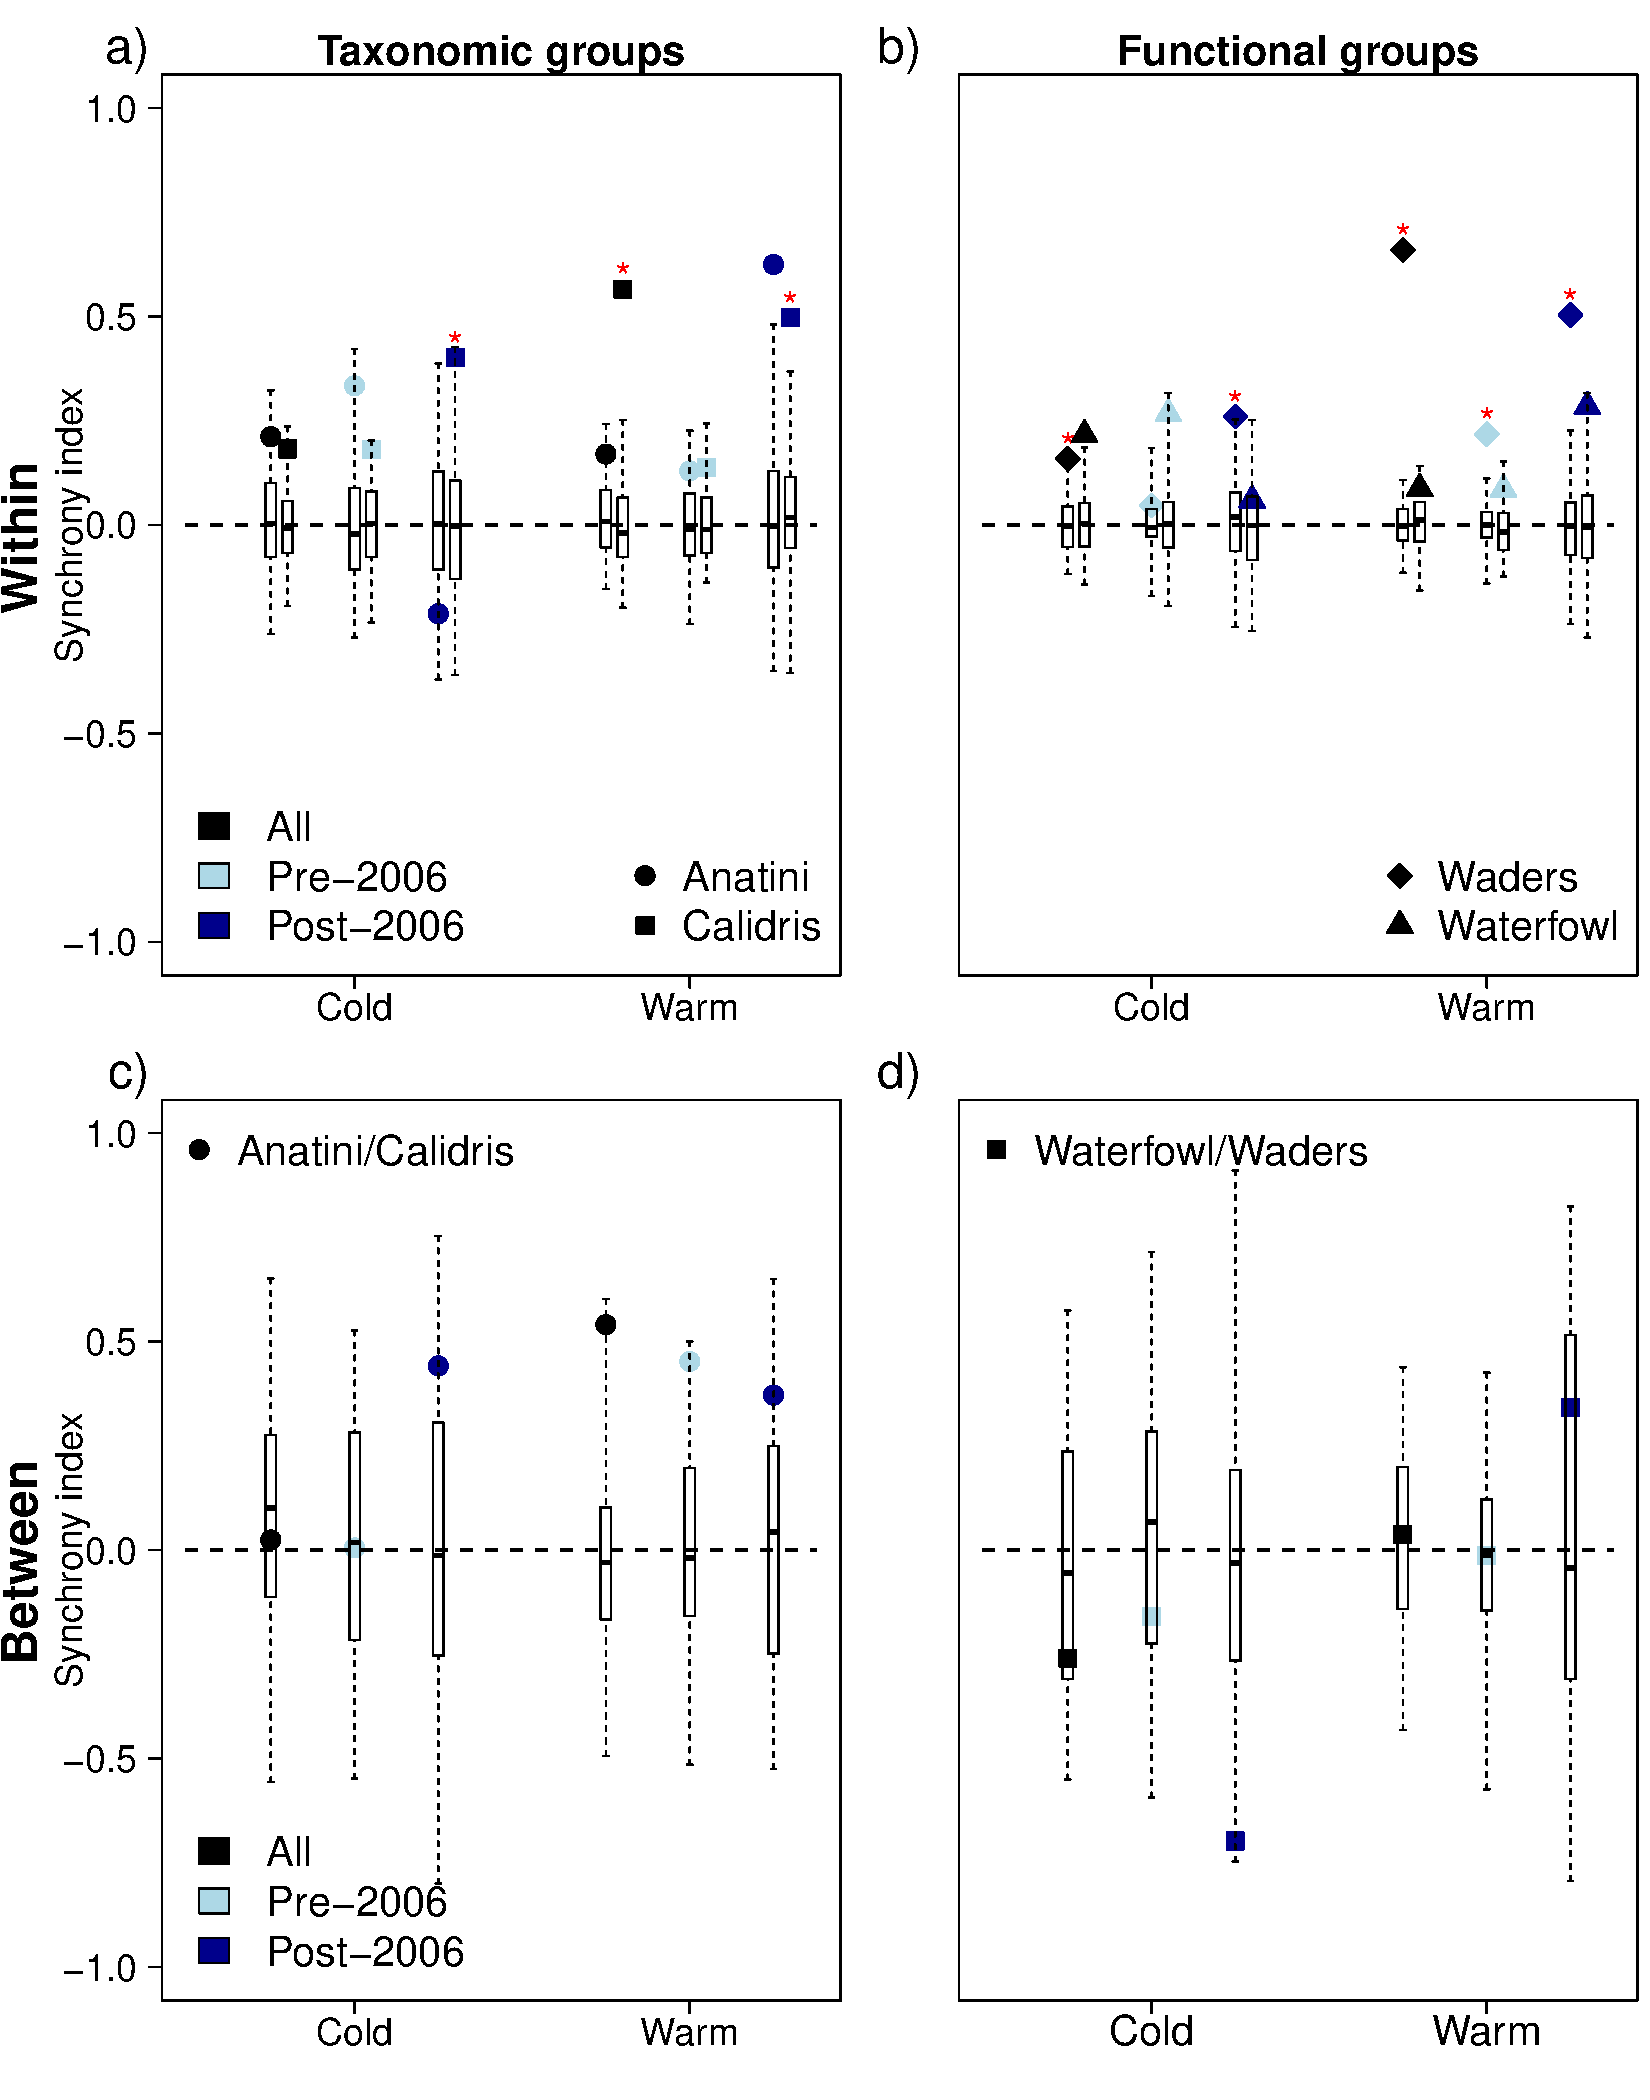
\includegraphics[width=0.85\textwidth]{Fig2_new3_JAE_abundances}
\par\end{centering}
\caption{Gross' synchrony index ($\eta$) as a function of the season (cold
and warm seasons), calculated \emph{within} (top, a-b) and \emph{between}
(bottom, c-d) groups. The groups considered were different functional
groups (waders vs waterfowl, right b-d) or taxonomic groups (\emph{Anatini},
\emph{Calidris}, left a-b). The index was computed in each panel on
the whole dataset (black) or using two periods: before and after 2006
(light and dark blue), the year of the change in water level management.
Boxplots indicate the distribution of $\eta$ under the null hypothesis
(independent species) and filled symbols correspond to the observed
values. Red stars correspond to synchrony values significantly different
from the null model, at the 10\% threshold with a Benjamini-Hochberg
correction. \label{fig:Gross-synchrony-index}}
\end{figure}

There are therefore contrasted results regarding the effect of the
management change on synchrony within guilds or within the whole bird
community. At the yearly (season) timescale, the results are unclear
for both guilds. At shorter (a few months) and longer (several years)
timescales though, the management change may decrease synchrony and
even promote compensation. 
\begin{figure}[H]
\begin{centering}
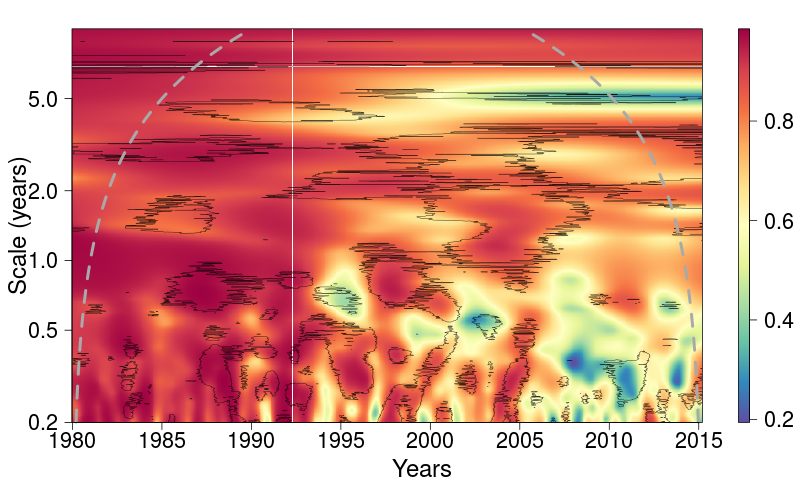
\includegraphics[width=0.95\textwidth]{Figure3_BH}
\par\end{centering}
\caption{Wavelet modulus ratio for the wader community, scaling from 0 (compensation,
blue color) to 1 (synchrony, red color). Black lines delineate regions
significantly different from the null model (independently fluctuating
species) with a false discovery rate controlled at the 10\% threshold.
\label{fig:Wavelet-modulus-ratio}}
\end{figure}


\subsection*{Synchrony between phylogenetic or functional groups}

More interpretable results can be found when we examine synchrony
vs compensation between functional groups (Fig. 2d). Since we consider
only two functional or phylogenetic groups, the Gross index reduces
to a simple correlation between two groups. \emph{Anatini} and \emph{Calidris}
are positively correlated in the warm season (for all periods), and
have unclear correlations during the cold season (Fig. 2c). In contrast,
waders and waterfowl are negatively correlated during the cold season
and positively correlated during the warm season (Fig. 2d). Although
the negative correlation is not statistically significant, it is consistent
for both pre- and post-2006 periods.

\subsection*{Synchrony in a small module with known competition}

Compensation could be expected upon visual inspection of the time
series of the two groups formed by cormorant on the one hand, and
little egret plus grey heron (summed as a small functional group)
on the other hand (Fig. \ref{fig:Time-series-of}, though see Appendix
S4 for alternative representations). However, we see on Fig. \ref{fig:Time-domain-(top)-and}
that synchrony is in fact the rule around the annual scale and below,
when considering the wavelet index. We wondered if the patterns in
Fig. \ref{fig:Time-series-of} were caused by the use of a log scale,
but we found that in fact the correlation was higher rather than lower
on the log scale (Appendix S4). However, over long temporal scales
($\sim$ 6 years) there seems to be some compensation, which could
correspond to the progressive change in composition within this small
community module, that was already visible on the abundance time series
plot (Fig. \ref{fig:Time-series-of}). There might be some compensation
over very short timescales as well (within the season), but at very
specific times.

\begin{figure}[H]
\begin{centering}
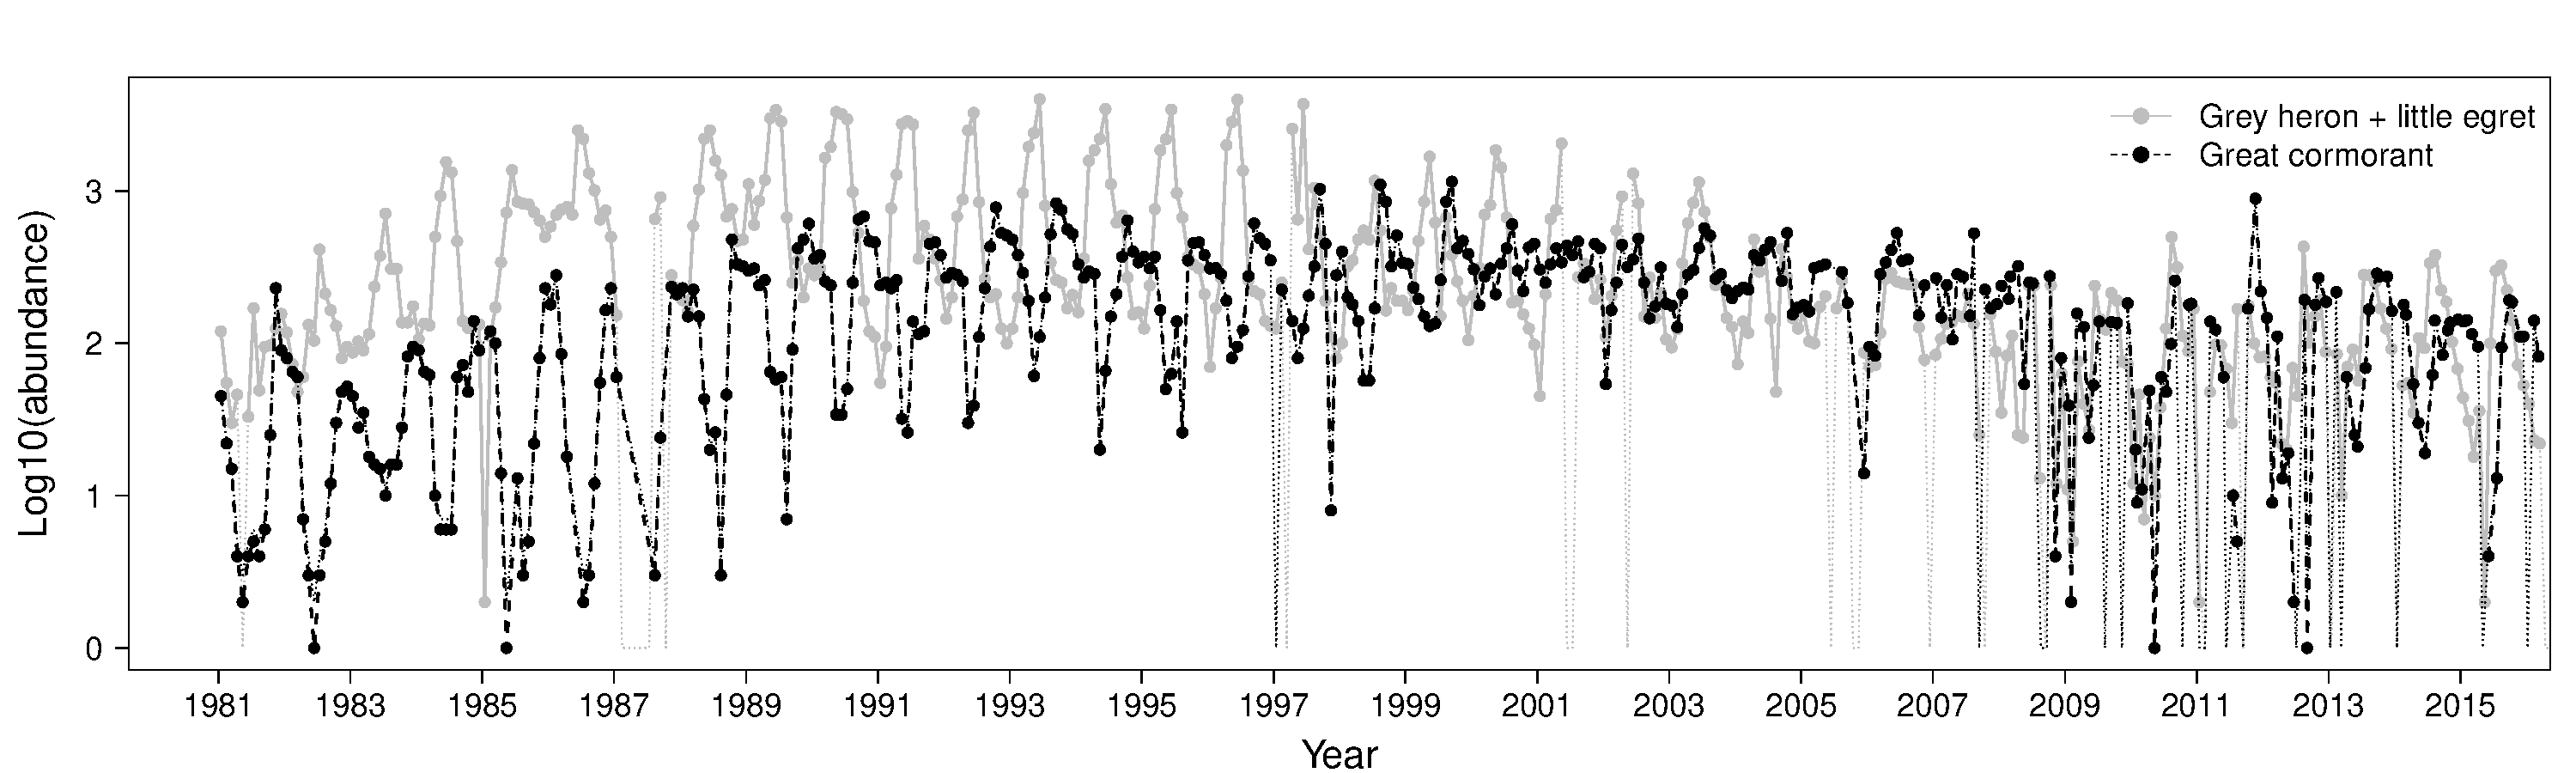
\includegraphics[width=1.1\textwidth]{abundance_3species}
\par\end{centering}
\caption{Time series of great cormorant abundance (dash-dotted black line),
as well as summed abundances of grey heron and little egret (solid
grey line). \label{fig:Time-series-of}}
\end{figure}

\begin{figure}[H]
\begin{centering}
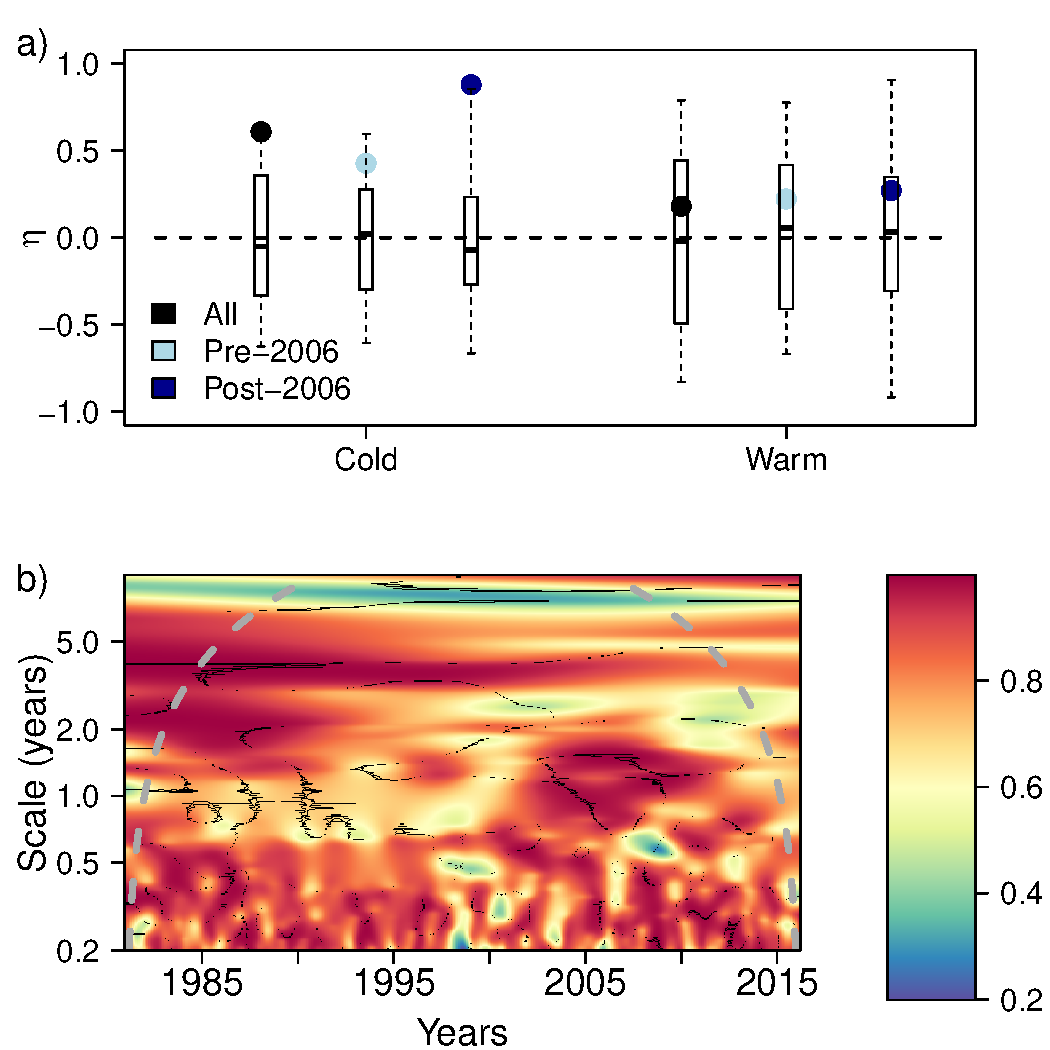
\includegraphics[width=0.99\textwidth]{triad_synchrony_2panels}
\par\end{centering}
\caption{Time-domain (a) and frequency-domain (b) synchrony analyses of the
group formed by cormorant, egret and heron (see the captions of Fig.
\ref{fig:Gross-synchrony-index} and Fig. \ref{fig:Wavelet-modulus-ratio}
for symbol interpretation) \label{fig:Time-domain-(top)-and}}
\end{figure}


\section*{Discussion}

Compensation was overall very rare at the yearly timescale (differentiating
between the cold and warm season), with synchrony between species
being the rule. In other words, there was no widespread ``functional
compensation'' (\textit{sensu} \citealt{gonzalez2009causes}) \emph{within}
genera or guilds at the annual scale or below. Yet, summing species
abundances within a guild and comparing the total abundance of contrasted
guilds, it was possible to find compensation (although the null hypothesis
of no correlation could not be rejected); in other words, there was
some compensation \emph{between} guilds. A zoom on a module of three
species with known competition also revealed compensation at scales
above 5 years. Similar results have been obtained using biomass in
place of abundance (Appendix S5). We elaborate below on these findings.

\subsection*{Synchrony \emph{within} or \emph{between} guilds}

Given that we compare the level of synchrony/compensation within guilds
(with many species) and between guilds (with only a handful of groups),
we checked in Appendix S6 if changing the number of ``compartments''
($n$) in the Gross $\eta$ index could affect its value. It did not
have marked effects, unless the number of compartments is equal to
2, in which case, significance is hard to achieve and some compensatory
dynamics can be missed with weak environmental response. However,
we found that if two guilds respond in opposite ways to a shared driver,
the stronger the response to the driver, the lesser the compensation
indicated by $\eta$ at the whole community level. This might explain
the low levels of compensation that we found at the overall wetland
bird community level (Appendix S3), in spite of the clear presence
of two guilds (waders and waterfowl) reacting in opposite way to a
shared driver (here, water levels). Analyses at several taxonomic/functional
scales are therefore warranted to be conclusive about compensation.

We used correlation between the summed abundances of closely related
species (species within the \textit{Anatini }\textit{\emph{tribe}}
vs species within the \textit{Calidris} genus) or the summed abundances
of functionally similar species (waders vs waterfowl) to uncover compensation.
The functional group classification produced some compensation between
guilds while the taxonomic classification did not, despite the contrasted
habitat preferences of these two phylogenetic groups. Using functional
groups produced more logical results, although as we stressed above,
due to the low power of the tests, the null hypothesis of no compensation
at the yearly scale is still plausible as well.

We expected to see compensation at the ``functional group scale''
irrespective of the season, because the requirements of these birds
are different, but waders and waterfowl were found to correlate negatively
only during the cold (wintering) season. This can be explained by
a broad inflow of birds in the summer, including non-resident individuals
that add random variation to the community dynamics (though other
explanations are possible).

It may be better to say that we detected ``compensation'' rather
than ``compensatory dynamics'' between bird species \citep{gonzalez2009causes}
as the observed long-term changes in species composition (more waders,
proportionally less waterfowl; Appendix S2) might be due to an increased
inflow of birds preferring low water levels (waders), and outflow
of birds preferring high water levels (waterfowl), under an overall
space constraint. In other words, the shift in community dynamics
is likely not directly due to births and deaths. However, it would
be incorrect to conclude that such local compensation is disconnected
from regional-scale community dynamics: which species are present
in the reserve affects their reproductive success, which feeds back
into regional-scale dynamics, and in turn, regional-scale dynamics
influence which species are locally settling and competing.

\subsection*{Effect of the change in management on synchrony}

Although we performed first analyses on the whole time series, a marked
change in management occurred around 2006, after which the water levels
were kept at a lower level. We have therefore also performed yearly
analyses pre- and post-2006. These showed very little differences
during either the warm or cold season. However, in the wavelet analyses,
we see at monthly or 5-year timescales more compensation after 2006.
Since the water levels are on average more appropriate for waders
and their overall proportion has increased, it may be tempting to
interpret this as a consequence of the community becoming saturated
with waders, but we caution that it is difficult to make any strong
conclusion based on a single synchrony index. Similar analyses on
beetle communities by \citet{klink_functional_2019} found little
effect of disturbances on synchrony patterns, even though in theory
such disturbances should promote synchrony. In fact, like us, they
might have found a little less synchrony after disturbance, but the
results were not clear cut. We now describe a case where the biological
processes at hand are better understood.

\subsection*{Synchrony in a small module with known competition}

Zooming in on the cormorant-heron-egret module, for which we knew
beforehand that competition for resting and roosting sites in the
summer season occurs between, on the one hand, cormorants, and on
the other hand, little egrets and grey herons (C. Feign�, pers. obs.).
Abundance time series suggested some negative correlation, but it
was not found on the annual scale for which synchrony (or an absence
of relation) dominates. Instead, we find that compensation mostly
occurs above the annual temporal scale, approximatively on a scale
of 6 years, much above the annual scale. This may indeed be a consequence
of the slow shift in frequencies cormorants and little egrets / grey
herons.

\subsection*{Conclusion and perspectives for theory}

Overall, our results suggest to search for compensation more often\emph{
between} rather than \emph{within} functional groups, and over relatively
long timescales, above the typical temporal autocorrelation of the
dominant driver (e.g., above 5 years if the main driver is a seasonal
climate). This rejoins the recent findings of \citet{klink_functional_2019}
who found that increased functional differences between species tend
to decrease synchrony. Our suggestion goes against calls to search
for compensation within closely related species but at very short
timescales \citep{vasseur2007spectral,gonzalez2009causes}, below
the timescale of the main synchronizing seasonal environmental driver,
in order to filter out its synchronizing effect. Although searching
for compensation at temporal scales below the seasonal abiotic driver
(e.g., temperature) was partly motivated by studies on plankton whose
community dynamics are much faster, with much shorter generation times,
we could have expected compensation to manifest also at that scale
(e.g., monthly). Indeed, movement of birds reacting to food availability
can certainly occur within the season, and wetlands have a finite
carrying capacity, so that there is competition for space, which could
promote short-term compensation. We suspect that instead, because
many species share common abiotic and biotic drivers (e.g., disturbances
due to nearby hunting) even below the yearly timescale, their dynamics
are bound to be synchronized to some degree.

The attractor of community dynamics, i.e., the shape of community
trajectories in phase space, seems to be more or less an annual cycle
here: the dominant species fluctuate seasonally, but even though there
are shifts in some species dynamics, no abundant species seem to exhibit
violent multi-year oscillations. If we had to describe our community
mathematically, a dynamical model with a stable fixed point forced
by seasonality and some noise would probably be appropriate. This
mild fluctuation scenario somehow contrasts with the dynamics of other
communities, such as insect pests, that have quite often multi-year
cycles (on top of seasonal cycles, for multivoltine species), with
possibly strong indirect interactions between similar species mediated
by predators and parasitoids \citep{murdoch2003consumer}. In this
latter context of internally-generated variability (``Endogenous
compensatory cycles\textquotedbl{} in \citealp{gonzalez2009causes}),
compensation is quite likely as well. \citet{klapwijk2018transient}
recently reported only transient synchrony between species of moths,
so that compensation could occur more frequently for more strongly
oscillating species. Therefore, compensation could be more likely
for those groups at the yearly timescale. Whether or not these findings
have some generality remains to be investigated by examining multi-species
synchrony for more varied animal taxa.

In many ways, searching for abundance compensation using biodiversity
time series data is searching for needles in a haystack: only some
specific temporal and functional/taxonomic scales allow to see compensation
whilst numerous confounding factors make the community co-vary positively
at all other scales \citep{vasseur_synchronous_2014}. Although the
knowledge of specific biological mechanisms increasing the densities
of some species at the expense of others can help, synchrony will
likely dominate community-level time series data for closely related
species, even in species that compete strongly \citep{ranta_detecting_2008,loreau_species_2008}.
This is true even in cases of known mechanisms of competition for
space or shifts in community composition due to abiotic changes affecting
differentially species preferences, as in this study. We therefore
suggest that ``zooming out'' functionally (considering summed abundances
of dissimilar functional groups) and temporally (considering temporal
scales well above the periodicity of the dominant abiotic driver)
may often be the best strategy to see the compensation that will inevitably
manifest if the community-level biomass is to be maintained within
bounds in the long run.

\subsection*{Acknowledgements}

We thank the birdwatchers and staff of the Teich Reserve/Landes Gascogne
regional park who contributed to data collection over the years, as
well as LPO Aquitaine for helping us retrieve the raw data. Constructive
feedback by the two referees, Roel van Klink and Mike Fowler, considerably
improved the manuscript. The data collection was supported by the
Landes Gascogne regional park as well as the Teich municipality, while
data analysis was funded by LabEx COTE (ANR-10-LABX-45). \\

}\end{linenumbers}

\bibliographystyle{ecology}
\bibliography{BiblioTeich}

\end{document}
